\documentclass{standalone}
\usepackage{tikz}
\definecolor{lightgreen}{RGB}{127,255,127}
\begin{document}


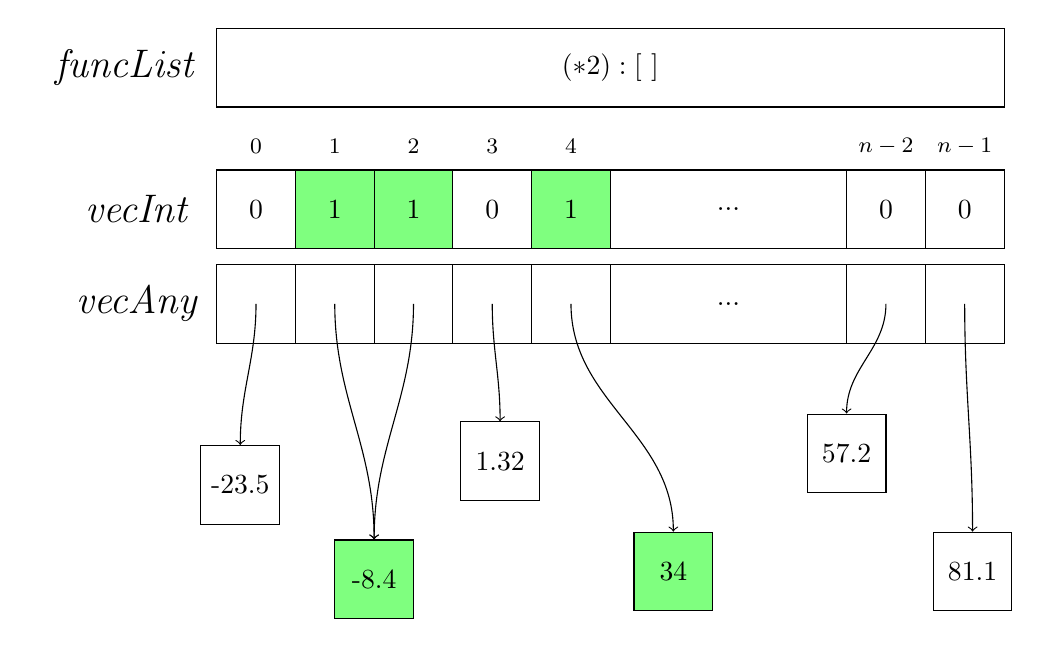
\begin{tikzpicture}

%\node[minimum size=1cm,draw] at (0,3) {$(+7)$};
%\node at (0.7,3) {:};
%\node[minimum size=1cm,draw] at (1.4,3) {$(*2)$};
%\node at (2.1,3) {:};
%\node at (2.8,3) {$[\ ]$};
\node[minimum width=2.5cm,align=right] at (-1.5,0) {\emph{\Large vecAny}};
\node[minimum width=2.5cm,align=right] at (-1.5,1.2) {\emph{\Large vecInt}};
\node[minimum width=2.5cm,align=right] at (-1.65,3) {\emph{\Large funcList}};

\node[minimum width=10cm,minimum height=1cm,draw] at (4.5,3) {$(*2) : [\ ]$};
%\node[minimum width=10cm,minimum height=1cm,draw] at (4.5,3) {$(+7) : (*2) : [\ ]$};

\node[minimum size=1cm,draw] at (0,1.2) {0};
\node[minimum size=1cm,draw,fill=lightgreen] at (1,1.2) {1};
\node[minimum size=1cm,draw,fill=lightgreen] at (2,1.2) {1};
\node[minimum size=1cm,draw] at (3,1.2) {0};
\node[minimum size=1cm,draw,fill=lightgreen] at (4,1.2) {1};
\node[minimum size=1cm,minimum width=3cm,draw] at (6,1.2) {...};
\node[minimum size=1cm,draw] at (8,1.2) {0};
\node[minimum size=1cm,draw] at (9,1.2) {0};

\node[minimum size=1cm,draw] at (0,0) {};
\node[minimum size=1cm,draw] at (1,0) {};
\node[minimum size=1cm,draw] at (2,0) {};
\node[minimum size=1cm,draw] at (3,0) {};
\node[minimum size=1cm,draw] at (4,0) {};
\node[minimum size=1cm,minimum width=3cm,draw] at (6,0) {...};
\node[minimum size=1cm,draw] at (8,0) {};
\node[minimum size=1cm,draw] at (9,0) {};

\node[minimum size=1cm,draw] (a) at (-0.2,-2.3) {-23.5};
\node[minimum size=1cm,draw,fill=lightgreen] (b) at (1.5,-3.5) {-8.4};
\node[minimum size=1cm,draw] (c) at (3.1,-2.0) {1.32};
\node[minimum size=1cm,draw,fill=lightgreen] (d) at (5.3,-3.4) {34};
\node[minimum size=1cm,draw] (e) at (7.5,-1.9) {57.2};
\node[minimum size=1cm,draw] (f) at (9.1,-3.4) {81.1};

\draw[->] (0,0) to [out=270,in=90] (a);
\draw[->] (1,0) to [out=270,in=90] (b);
\draw[->] (2,0) to [out=270,in=90] (b);
\draw[->] (3,0) to [out=270,in=90] (c);
\draw[->] (4,0) to [out=270,in=90] (d);
\draw[->] (8,0) to [out=270,in=90] (e);
\draw[->] (9,0) to [out=270,in=90] (f);

\node at (0,2) {\footnotesize 0};
\node at (1,2) {\footnotesize 1};
\node at (2,2) {\footnotesize 2};
\node at (3,2) {\footnotesize 3};
\node at (4,2) {\footnotesize 4};
\node at (8,2) {\footnotesize $n-2$};
\node at (9,2) {\footnotesize $n-1$};
\end{tikzpicture}


\end{document}
